\documentclass[memoire.tex]{subfiles}
\begin{document}
\chapter{Etat de l'art}
Le clustering est le regroupement de plusieurs données similaires en un seul groupe appelé cluster. L'analyse de cluster permet ainsi d'identifier des groupes de données relativement homogènes sur la base de leur similarité pour des caractéristiques données ce qui dans notre cas peut par exemple être le type d'emploi occuper en fonction des filières suivies par d'anciens étudiants. Cependant analyser différents profils d'individus peut représenter des difficultés techniques importantes, c'est pourquoi cette première section du document présentera les différentes solutions possibles pouvant apporter une réponse à cette difficulté de catégorisation des parcours. 
	\section{Les types de clustering}
		\subsection{Clustering hiérarchique}
Parmis les différents types de clustering existant \cite{ref4}, le premier étudié sera le clustering hiérarchique. Très utilisé comme outil d'analyse de données, l'idée principale de cette méthode est de construire un arbre binaire fusionnant de façon successive les groupes de points similaires. L'un des avantages de cette méthode est tout d'abord l'apport de l'arbre qui permet d'avoir une vision globale des données traitées. De plus, cette méthodologie possède ses propres outils de visualisation qui sont le dendrogramme et la classification double. Le dendrogramme permet d'illustrer l'arrangement des clusters (figure 1.1)\cite{ref8} :
\begin{itemize}
\item la racine de l'arbre est formée par un cluster contenant l'ensemble des objets.
\item chaque noeud de l'abre consitute un cluster.
\item l'union des objets des noeuds fils correspond aux objets présent dans ce noeud.
\item les paliers sont indéxés en fonction de l'ordre de construction.
\end{itemize}
 Tandis que la classification double est une technique d'exploration de données non-supervisée permettant de segmenter simultanément les lignes et les colonnes d'une matrice. L'autre avantage du clustering hiérarchique est sa facilité d'implémentation dans des algorithmes tel que K-Means en plus de fournir une représentation comme dit précédemment. Afin d'établir un arbre hiérarchique, le clustering hiérarchique à recours à deux méthodes qui sont la méthode agglomérative et la méthode divisive. Un regroupement agglomératif traite chaque objet comme un seul élément qui à chaque étape de l'algorithme est fusionné avec un second objet présentant le plus de similarités en un nouveau cluster de plus grande taille. Ce processus est répété jusqu'à que ce que tous les points soient membre d'un seul et même cluster. A l'inverse d'un regroupement agglomératif qui utilise une approche "bottom-up", les algorithmes divisifs utilisent une approche "top-down". Ces algorithmes débutent ainsi leur traitement à partir de la racine de l'arbre ou tous les objets sont regroupés en un seul cluster. A chaque ittération les cluster les plus hétérogènes sont divisés en deux jusqu'à ce que l'ensemble des objets fassent parti de leur propre cluster.Cependant sa complexité le rend inefficace sur de larges jeux de données \cite{ref7}. De plus, la première injection de données ainsi que l'ordre de celles-ci  à un fort impact sur le résultat final. En outre, il n'est pas possible de défaire ou modifier les étapes précédentes du traitement, c'est à dire qu'une fois une instance assignées à un cluster, il n'est plus possible de la déplacée pour effectuer d'éventuelles modifications ou corrections \cite{ref5}. Dans notre cas la base de CV utilisée n'étant pas de taille importante le clustering hiérarchique reste une méthode applicable. Cependant la problématique à résoudre est la gestion des filières intégrant plusieurs domaines tel que la filière MIASHS de Nanterre qui possède une dimension mathématiques et une informatique. Les données étant représentées sous forme d'arbre cela entrainerait une répétition au niveau des résultats.
	\begin{figure}
		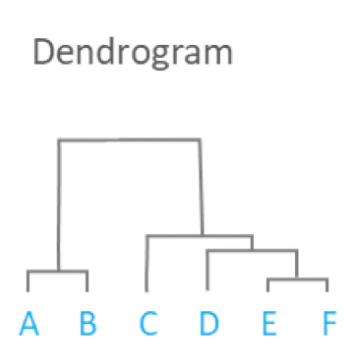
\includegraphics[scale=0.8]{img/hierarchical_clustering.png}
		\caption{Exemple de dendrogramme}
	\end{figure}
	
\newpage
\subsection{Le clustering par partionnement}
Le clustering par partionnement contrairement au clustering hiérarchique qui utilise un arbre afin de représenter les différents groupe de données va classifier les différents objets en groupe en fonction de leur similarités. Cependant ce mode de fonctionnement pause un problème concernant le choix de la "bonne représentation" en fonction d'un critère choisi, le but devient alors de recherche une représentation optimale de son critère à travers plusieurs itérations.\cite{ref8} L'algorithme le plus utilisé pour ce type de méthode est K-means qui sera présenté dans la suite de ce document.

\section{Les types de clusters}

Le but du clustering étant de trouver des groupes d'objets présentant des similarités
définies en fonction de l'objectif recherché. Il existe toutefois une multitude de types de cluster qui seront étudiés au sein de cette section chacun avec ses avantages et inconvénients en fonction de notre cas avant de statuer sur le type qui sera utilisé pour le reste de ce document.

\subsection{Well-Separated}
Un cluster "well-separated" est un regroupement de points de telle façon à ce que tous les points faisant parti d'un même cluster présentent de fortes similarités entre eux comparés aux points d'un cluster extérieur.
\subsection{Prototype-Based}

Un prototype-based cluster est un cluster dont les points qui le constitue sont plus proches ou similaire du prototype définissant le cluster traité que de tout autre prototype définissant d'autres clusters.

\subsection{Graph-Based}
Le graph-based cluster est utilisé dans les cas ou les données peuvent être représenté sous forme de graphe dont les nœuds sont des objets et les liens représentent les connexions entre ceux-ci. Dans cette situation un cluster peut être défini comme un composant connecté,  c'est-à-dire un groupe d'objets liés les uns aux autres au sein du même groupe.

\subsection{Density-Based}
A travers l'utilisation d'un density-based cluster, le but est de détecter les zones ou les points formant des clusters sont concentrés et celles ou les points sont séparés par des zones vides ou par des zones contenant très peu de points. Les points ne faisant par partie d'un agrégat sont ici classés comme du bruit.


\newpage
\section{Les algorithmes}
Dans cette section seront décrit les principaux algorithmes utilisés lorsque des techniques de clustering sont employées. Les avantages et inconvénients de chacun seront présentés en fonction du cas présenté dans l'introduction.
\subsection{K-means}

L'algorithme K-means est l'algorithme le plus populaire, celui-ci recherche la meilleure division possible au sein d'un jeux de données \cite{ref5} en plus de sa facilité d'implémentation. Cependant celui-ci impose de savoir le nombre de clusters souhaités et par conséquent une bonne connaissance des données utilisées.

\subsection{Agglomerative Hierarchical Clustering}

Les techniques de clustering agglomératives partent d'un ensemble de points formant un cluster, par la suite, les deux clusters les plus proches sont fusionnés successivement jusqu'à ce qu'il n'y est plus qu'un seul cluster restant. \cite{ref4}

\subsection{DBSCAN}

DBSCAN est un algorithme basé sur le partitionnement de données, celui-ci utilise deux principaux paramètres qui sont la distance et le nombre de points minimum devant se trouver dans un rayon donné afin qu'ils soient considérés comme un cluster.
\end{document}